\documentclass[]{book}
\usepackage{lmodern}
\usepackage{amssymb,amsmath}
\usepackage{ifxetex,ifluatex}
\usepackage{fixltx2e} % provides \textsubscript
\ifnum 0\ifxetex 1\fi\ifluatex 1\fi=0 % if pdftex
  \usepackage[T1]{fontenc}
  \usepackage[utf8]{inputenc}
\else % if luatex or xelatex
  \ifxetex
    \usepackage{mathspec}
  \else
    \usepackage{fontspec}
  \fi
  \defaultfontfeatures{Ligatures=TeX,Scale=MatchLowercase}
\fi
% use upquote if available, for straight quotes in verbatim environments
\IfFileExists{upquote.sty}{\usepackage{upquote}}{}
% use microtype if available
\IfFileExists{microtype.sty}{%
\usepackage{microtype}
\UseMicrotypeSet[protrusion]{basicmath} % disable protrusion for tt fonts
}{}
\usepackage[margin=1in]{geometry}
\usepackage{hyperref}
\hypersetup{unicode=true,
            pdftitle={Zygolabs: Zygomycete Fungi In Teaching And Research},
            pdfauthor={Joseph W. Spatafora, Ying Chang, Jason E. Stajich, Derreck Carter-House, Yan Wang, Matthew E. Smith, Nicole Reynolds, Tim James, Kevin Amses, William Davis, Merlin White, Greg Bonito, Jessie Uehling, Robert Roberson},
            pdfborder={0 0 0},
            breaklinks=true}
\urlstyle{same}  % don't use monospace font for urls
\usepackage{natbib}
\bibliographystyle{apalike}
\usepackage{longtable,booktabs}
\usepackage{graphicx,grffile}
\makeatletter
\def\maxwidth{\ifdim\Gin@nat@width>\linewidth\linewidth\else\Gin@nat@width\fi}
\def\maxheight{\ifdim\Gin@nat@height>\textheight\textheight\else\Gin@nat@height\fi}
\makeatother
% Scale images if necessary, so that they will not overflow the page
% margins by default, and it is still possible to overwrite the defaults
% using explicit options in \includegraphics[width, height, ...]{}
\setkeys{Gin}{width=\maxwidth,height=\maxheight,keepaspectratio}
\IfFileExists{parskip.sty}{%
\usepackage{parskip}
}{% else
\setlength{\parindent}{0pt}
\setlength{\parskip}{6pt plus 2pt minus 1pt}
}
\setlength{\emergencystretch}{3em}  % prevent overfull lines
\providecommand{\tightlist}{%
  \setlength{\itemsep}{0pt}\setlength{\parskip}{0pt}}
\setcounter{secnumdepth}{5}
% Redefines (sub)paragraphs to behave more like sections
\ifx\paragraph\undefined\else
\let\oldparagraph\paragraph
\renewcommand{\paragraph}[1]{\oldparagraph{#1}\mbox{}}
\fi
\ifx\subparagraph\undefined\else
\let\oldsubparagraph\subparagraph
\renewcommand{\subparagraph}[1]{\oldsubparagraph{#1}\mbox{}}
\fi

%%% Use protect on footnotes to avoid problems with footnotes in titles
\let\rmarkdownfootnote\footnote%
\def\footnote{\protect\rmarkdownfootnote}

%%% Change title format to be more compact
\usepackage{titling}

% Create subtitle command for use in maketitle
\newcommand{\subtitle}[1]{
  \posttitle{
    \begin{center}\large#1\end{center}
    }
}

\setlength{\droptitle}{-2em}

  \title{Zygolabs: Zygomycete Fungi In Teaching And Research}
    \pretitle{\vspace{\droptitle}\centering\huge}
  \posttitle{\par}
    \author{Joseph W. Spatafora, Ying Chang, Jason E. Stajich, Derreck Carter-House,
Yan Wang, Matthew E. Smith, Nicole Reynolds, Tim James, Kevin Amses,
William Davis, Merlin White, Greg Bonito, Jessie Uehling, Robert
Roberson}
    \preauthor{\centering\large\emph}
  \postauthor{\par}
      \predate{\centering\large\emph}
  \postdate{\par}
    \date{2019-04-09}

\usepackage{booktabs}
\usepackage{amsthm}
\makeatletter
\def\thm@space@setup{%
  \thm@preskip=8pt plus 2pt minus 4pt
  \thm@postskip=\thm@preskip
}
\makeatother

\begin{document}
\maketitle

{
\setcounter{tocdepth}{1}
\tableofcontents
}
\chapter*{Preface}\label{preface}
\addcontentsline{toc}{chapter}{Preface}

ZyGoLife is an interdisciplinary research consortium focused on
advancing research and education of zygomycete fungi. ZyGoLife is funded
by the National Science Foundation as part of the Genealogy of Life
Program (DEB-1441604, DEB-1441715, DEB-1441677, DEB-1441728). It is
based in numerous laboratories and institutions with research expertise
in systematics, ecology, cell biology, genomics, and evolutionary
biology.

Zygomycetes are an important group of fungi with respect to evolutionary
origins of terrestrial fungi, ecological processes in nature, and
industrial uses by humans. They are, however, one of the more
understudied groups of fungi. To advance the study of zygomycetes,
ZyGoLife is producing \emph{ZyGoLabs: Zygomycete Fungi in Teaching and
Research}. It is our hope that this effort will advance teaching and
research of zygomycetes, and that it will entice more teachers to
incorporate them in the classroom and more mycologists -- professors and
students alike -- to study them. The title of the book is an homage to
\emph{Zoosporic Fungi in Teaching and Research}, which is how many of us
first learned the mycology of flagellated fungi.

This version of \emph{ZyGoLabs: Zygomycete Fungi in Teaching and
Research} is a prelease draft and served as the basis for the ZyGoLife
Workshop held at the annual Mycological Society of America meeting on
July 15, 2017 at the University of Georgia, Athens GA. It will be
further developed over the near future and released as a formal
publication.

\emph{ZyGoLabs: Zygomycete Fungi in Teaching and Research} is dedicated
to Gerald L. Benny, Kerry L. O'Donnell and Robert W. Lichtwardt. They
carried the torch in zygomycete fungi research over the past 40 years,
providing the foundation for today's researchers in zygomycete biology.
This publication and indeed the ZyGoLife research consortium would not
be possible without them.

\chapter{Overview of zygomycete fungi}\label{intro}

\emph{Joseph W. Spatafora}

Department of Botany and Plant Pathology, Oregon State University,
Corvallis, OR 97331

\section{Overview of Kingdom Fungi}\label{overview-of-kingdom-fungi}

Fungi are frequently described as four groups -- chytridiomycetes,
zygomycetes, ascomycetes and basidiomycetes -- that are defined by
morphologies associated with reproduction. The chytridiomycetes are
recognized based on their production of zoospores, characterized by a
single posterior, whiplash flagellum. The zygomycetes are characterized
by gametangial conjugation and the production of zygospores (Fig.
\ref{fig:zygomorph}a), aseptate (coenocytic) hyphae, and asexual
reproduction typically by sporangia (Fig. \ref{fig:zygomorph}b). The
ascomycetes and basidiomycetes are diagnosed by the production of asci
and basidia, respectively, possession of regularly septate hyphae, and a
dikaryotic nuclear phase in their life cycle. The classification of
Kingdom Fungi used here recognizes eight phyla (Fig. \ref{fig:ftol},
Table \ref{tab:fungal-class}) with the chytrids comprising three
paraphyletic lineages including Cryptomycota/Microsporidia,
Chytridiomycota and Blastocladiomycota. The zygomycetes are also
paraphyletic and are classified in two phyla, Zoopagomycota and
Mucoromycota. The monophyly of ascomycetes and basidiomycetes has been
confirmed and they are classified as phyla Ascomycota and Basidiomycota,
respectively, of the subkingdom Dikarya.

\section{Zygomycete fungi}\label{zygomycete-fungi}

Genome-scale phylogenies do not support the monophyly of zygomycetes and
reject the zygospore as a synapomorphy for them
(\citet{Spatafora_2016}). Rather the zygospore, as it is currently
defined, arose in the MRCA of Zoopagomycota, Mucoromycota, Ascomycota
and Basidiomycota, and lost in the MRCA of Dikarya
(Ascomycota+Basidiomycota). Most zygomycetes are characterized by
coenocytic hyphae and sporangial asexual reproduction, but lineages
exist that are characterized by septate or compartmentalized hyphae
(Fig. \ref{fig:zygomorph}c) and/or asexual reproduction by formation of
conidia (Fig. \ref{fig:zygomorph}d). Importantly, it is with the
emergence of the zygomycete fungi that we observe a loss of the fungal
flagellum and the rise of the terrestrial, filamentous fungi. It is
assumed that this loss of the flagellum in Kingdom Fungi corresponds to
the transition to terrestrial environment and the emergence of
terrestrial ecosystems.

\section{Zoopagomycota}\label{zoopagomycota}

Zoopagomycota is sister to Mucoromycota+Dikarya. It comprises three
subphyla, Zoopagomycotina, Kickxellomycotina and Entomophthoromycotina.
The primary ecologies of the phylum include pathogens and commensals of
animals, parasites of other fungi and amoebae, and rarely as plant
associates. The placement of Zoopagomycota as sister to the remainder of
nonflagellated fungi suggests that diversification with animals and
nonplant hosts occurred at least as early as diversification with
terrestrial plants. Also, the loss of the flagellum in fungi corresponds
to other modifications including the loss of the centriole. Most
nonflagellated fungi of Mucoromycota, Basidiomycota and Ascomycota
possess an organelle unique to fungi, the spindle pole body (SPB), which
serves as the microtubule organizing center necessary for chromosome
segregation during nuclear division. In contrast, Zoopagomycota lineages
retain a functional centrosome that possesses a degenerate 9+2
microtubular system (\citet{McLaughlin_2015}). There is some evidence
that \emph{Olpidium}, a genus of zoosporic fungus that retains its
flagellum and infects nematodes and plant roots of Brassicaceae, may be
closely related to Zoopagomycota (\citet{Sekimoto_2011}).

Zoopagomycotina contains a single order Zoopagales (Ch2, Ch3). Species
of the order include predators of nematodes (e.g., \emph{Stylopage}) and
nematode eggs (e.g., \emph{Rhopalomyces}), predators of amoebae (e.g.,
\emph{Stylopage}, \emph{Zoopage}), and mycoparasites of mucoralean fungi
(e.g., \emph{Syncephalis}). Hyphae are small in diameter, coenocytic,
and they form haustoria on or within their hosts. Asexual reproduction
is by conidia or sporangia according to species, and where known sexual
reproduction is by production of zygospores. Many of these fungi are
obligate symbionts and thus difficult to obtain in axenic culture, and
for this reason there exists a paucity of molecular and genomic data.

Kickxellomycotina comprises four orders, Asellariales, Dimargaritales,
Harpellales and Kickxellales (Ch2, Ch4). Species of Kickxellomycotina
possess hyphae that are regularly compartmentalized by bifurcate septa
that are occluded by a lenticular plug (Fig \ref{fig:zygomorph}c).
Asellariales and Harpellales (Ch4) are associated with digestive tracts
of aquatic stages of arthropods and comprise two of the four orders that
have been treated previously as Trichomycetes (Lichtwardt 1986); the
other two orders, Amoebidiales and Eccrinales, are members of
Mesomycetozoea, not Kingdom Fungi (\citet{Benny_2000},
\citet{Cafaro_2005}). Asellariales has filamentous, branched thalli and
reproduce asexually by disarticulation of the thalli into arthrospores
(Ch 4). They occur in the digestive tracts of marine, aquatic and
terrestrial species of isopods and Collembola where they are thought to
function as commensals. Harpellales has branched or unbranched
filamentous thalli and reproduce by trichospores, asexual spores with
hair-like appendages (Ch. 4). They attach to the hindgut of aquatic
stages of arthropods via a holdfast and are generally considered to be
in a commensal relationship with their host. Dimargaritales species are
haustorial parasites of other fungi with the best-known species
occurring on mucoralean hosts (\citet{Benjamin_1965}), and Kickxellales
(Ch 2) includes mycoparasites and saprobes isolated from soil. Both
Dimargaritales and Kickxellales produce unique sporangia called
merosporangia (Fig. \ref{fig:zygomorph}e). These are cylindrical
sporangia that arise from a bulbous structure, and one or more
sporangiospores may occur in chains within the sporangium.

Entomophthoromycotina (Ch. 5, Ch. 6) contains three classes each with a
single order: Basidiobolomycetes and Basidiobolales,
Entomophthoromycetes and Entomophthorales, and Neozygitomycetes and
Neozygitales (\citet{Humber_2012}, \citet{Benny_2014},
\citet{Spatafora_2016}). These fungi are associated with animals as
either commensals isolated from animal dung or as pathogens and
parasites of insects. Many species are commonly isolated from soil and
maintained in pure culture, which is consistent with a saprobic life
cycle phase. Basidiobolales is typically isolated from amphibian dung
although species are known to occur on the dung of other vertebrates.
They produce conidiophores that forcibly eject a primary conidium, which
if it lands on an appropriate substrate will germinate to form a
mycelium, or if not, undergo repetitive germination, producing a second
conidium (Ch 6). Under some conditions nonforcibly discharged
capilliconidia are produced from forcibly discharged primary conidia.
Capilliconidia adhere to the outer surface of insects. Dispersal is then
achieved when spore-carrying insects are ingested by insectivorous
animals, and after surviving gut passage, the fungus is subsequently
excreted with the feces. The phylogenetic placement of Basidiobolales
with molecular and genome scale data is problematic. In all current
datasets, it is characterized by long and unstable branches and its
relationship to other Entomophthoromycotina is unambiguous at this time
(\citet{Gryganskyi_2012}). Entomophthorales, literally, insect
destroyers, comprises pathogens of insects. Like Basidibolales, they
also produce forcibly discharged conidia (Ch 5). They infect their hosts
via spores and multiply within the host as one to two-celled hyphal
bodies, which also can function as gametangia. Upon the host's death,
the fungus ruptures through the cuticle segments producing forcibly
discharged primary conidia. Frequently, infected hosts alight in perched
or elevated positions, a phenomenon known as summit disease, which is
thought to be an induced behavior or adaptation for spore dispersal of
the pathogen (\citet{Gryganskyi_2017}). Neozygitales are pathogens of
insects and mites. They were classified as a family within
Entomophthorales, but were distinguished from Entomophthorales based on
shape and size of chromosomes (\citet{Humber_2012}), although inadequate
molecular data currently exist to test this hypothesis.
\emph{Neozygites} produces adhesive capilliconidia similar to that of
\emph{Basidiobolus.}

\section{Mucoromycota}\label{mucoromycota}

Mucoromycota consists of three subphyla including Glomeromycotina,
Mortierellomycotina and Mucoromycotina. Unlike Zoopagomycota,
Mucoromycota is characterized by plant associations and plant based
ecologies (e.g., mycorrhizae, root endophytes, decomposers, etc.). Some
do exist as parasites of animals and other fungi, but these all
represent opportunistic infections of hosts with compromised immune
systems or relatively recent derivations from saprobic ecologies
(\citet{Hoffmann_2013}). Mucoromycota is the sister group to Dikarya,
which is also characterized by dominant plant associated life styles,
suggesting that the MRCA of Mucoromycota and Dikarya corresponds to the
origin of modern fungal-plant associations, or at least the evolutionary
potential for such relationships.

Glomeromycotina (Ch. 7) consists of the arbuscular mycorrhizae and
\emph{Geosiphon}, a symbiont of cyanobacteria (\citet{Redecker_2014}).
Arbuscular mycorrhizae are the most common form of mycorrhizae on the
planet, and arbuscule fossils are present among the first land plant
fossils (\citet{Taylor_2015}), confirming an ancient symbiosis. As such
they are a central taxon in the development of hypotheses concerning the
evolution of early land plants and terrestrial ecosystems. Despite this
importance, they have been an enigma with respect to phylogenetics of
Kingdom Fungi. Morphologically, they resemble zygomycetes in the
production of coenocytic hyphae and terminal or subterminal spores that
resemble azygospores, asexually formed zygospore-like structures
produced terminally on a single hypha or suspensor cell. Sexual
reproduction has never been observed for the group, preventing analysis
of morphological characters traditionally used in classifications. Early
molecular phylogenies based on the small subunit ribosomal DNA (SSU DNA)
resolved the arbuscular mycorrhizae -- with varying statistical support
depending on the analysis -- as separate from the zygomycetes and sister
to Dikarya (\citet{Sch_2001}). However, genome-scale phylogenies and
genome content analyses strongly support the arbuscular mycorrhizae as a
member of Mucoromycota (\citet{Spatafora_2016}). Currently there are
four orders of Glomeromycotina, Archaeosporales, Diversisporales,
Glomerales and Paraglomerales with \emph{Geosiphon} being classified in
Archaeosporales (\citet{Redecker_2014}).

The relationship of Glomeromycotina to the other subphyla of
Mucoromycota is unresolved, with some analyses resolving it as sister to
Mortierellomycotina+Mucoromycotina, while others resolve it as sister
group to Mortierellomycotina (\citet{Spatafora_2016}). The taxon
sampling for both Glomeromycotina and Mortierellomycotina is sparse and
expanded taxon sampling is needed to fully test these rival hypotheses.
Mortierellomycotina, and its sole order Mortierellales, are commonly
isolated soil fungi (Ch 8). They produce zygospores and sporangia
similar to some species of Mucorales, the order in which they were
previously classified, but molecular phylogenetics
(\citet{Hoffmann_2011}) and genome-scale (\citet{Spatafora_2016})
phylogenies both strongly support the taxon as representing a distinct
subphylum. These fungi have been demonstrated as root endophytes of
plants, but their effect on the host fitness remains unknown.
Mortierellales are also prolific producers of fatty acids, in particular
arachidonic acid. Both Glomeromycotina and Mortierellomycotina possess
intimate relationships with bacteria, and while facultative, show high
levels of specificity and cospeciation (\citet{Bonfante_2017}), the
fungus tends to grow better when cleared of the bacterium
(\citet{Uehling_2017}).

Mucoromycotina (Ch 9, Ch 10) contains the remainder of known zygomycete
species and is classified in three orders: Mucorales, Umbelopsidales and
Endogonales (\citet{Spatafora_2016}). Mucorales is one of the more
commonly isolated groups of fungi, as many are fast growing, early
colonizers of carbon rich substrates. Because many species culture
relatively easily, Mucorales are well represented in culture collections
and their zygospores and sporangia are well documented. They include
taxa that cause economically significant pre- and postharvest diseases
of fruits (e.g., \emph{Gilbertella, Mucor, Rhizopus}). They also
significantly impact humans both beneficially through their use in
industrial production of food (e.g., tempeh, \emph{Rhizopus}) and
compounds used as food supplements (e.g., beta-carotene,
\emph{Blakeslea}), and antagonistically as rare but increasingly
diagnosed human mycoses (e.g., \emph{Mucor, Apophysomyces}). It is among
Mucorales that sexual reproduction in fungi was first demonstrated and
numerous species of Mucorales exhibit phototropic responses to light
(Ch. 9, Ch. 10), making them important eukaryotic model organisms (e.g.,
\emph{Mucor mucedo, Phycomyces blakesleeanus}). Umbelopsidales was
recently described for \emph{Umbelopsis }(\citet{Spatafora_2016}), a
genus of soil-inhabiting fungi that also occurs as root endophytes.
Endogonales are saprobic or ectomycorrhizal depending on the species
(81). Saprobic species occur in heavily decayed woody substrates while
mycorrhizal species associate with both early diverging land plants and
vascular plants (Fig. \ref{fig:zygomorph}f, Bidartondo et al. 2011).
They have been argued as important organisms in the colonization of land
by green plants (Field et al. 2014) and represent an independent origin
of mycorrhizae relative to both Glomeromycotina and Dikarya.

\begin{figure}

{\centering 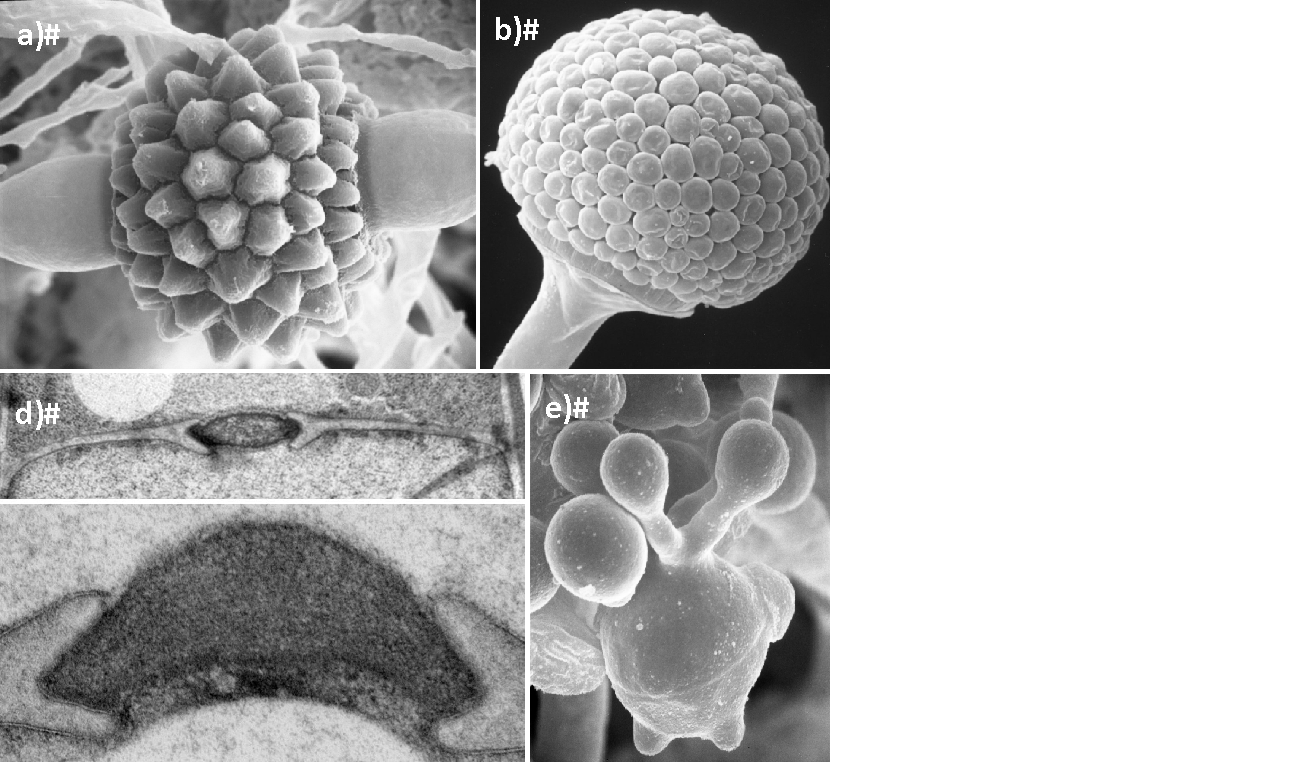
\includegraphics[width=17.49in]{img/Fig1_Ch1} 

}

\caption{Zygomycete morphologies. a) Zygosporangium of *Cunninghamella homothallica*. b) Sporangium of *Rhizopus stolonifer*. c) Merosporangium of *Kickxella alabastrina* d) Bifurcate septum with lenticular plug, *Coemansia*. e) Primary conidium of *Conidiobolus coronatus* with secondary microconidia. (Photos by K. O’Donnell, Zygomycetes in Culture.) f) Endogone flammicorona sporocarp, zygospores (inset)}\label{fig:zygomorph}
\end{figure}

\begin{figure}

{\centering 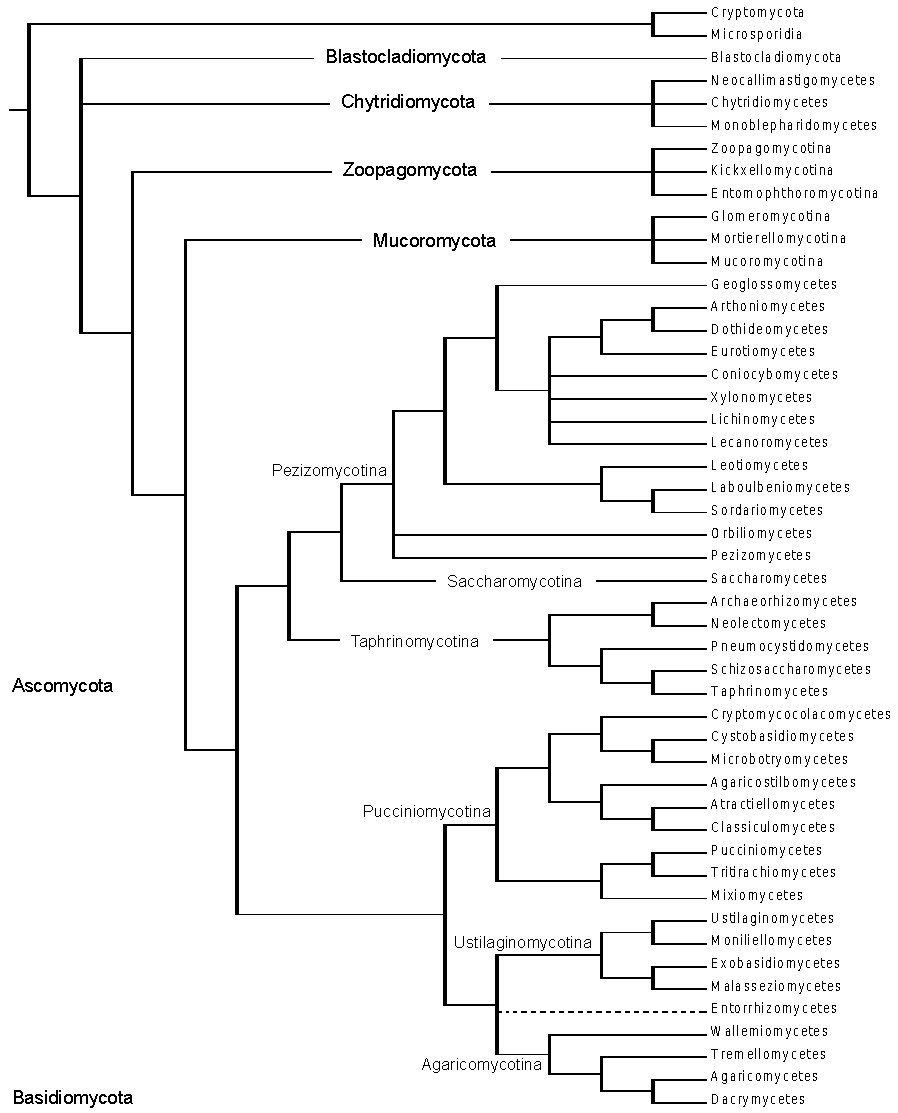
\includegraphics[width=11.97in]{img/Fig2_Ch1} 

}

\caption{Fungal Tree of Life}\label{fig:ftol}
\end{figure}

\begin{longtable}[]{@{}lll@{}}
\caption{\label{tab:fungal-class} Classification of Kingdom
Fungi.}\tabularnewline
\toprule
\begin{minipage}[b]{0.32\columnwidth}\raggedright\strut
Phylum\strut
\end{minipage} & \begin{minipage}[b]{0.28\columnwidth}\raggedright\strut
Subphylum\strut
\end{minipage} & \begin{minipage}[b]{0.31\columnwidth}\raggedright\strut
Class\strut
\end{minipage}\tabularnewline
\midrule
\endfirsthead
\toprule
\begin{minipage}[b]{0.32\columnwidth}\raggedright\strut
Phylum\strut
\end{minipage} & \begin{minipage}[b]{0.28\columnwidth}\raggedright\strut
Subphylum\strut
\end{minipage} & \begin{minipage}[b]{0.31\columnwidth}\raggedright\strut
Class\strut
\end{minipage}\tabularnewline
\midrule
\endhead
\begin{minipage}[t]{0.32\columnwidth}\raggedright\strut
\textbf{Cryptomycota} M.D.M. Jones \& T.A. Richards 2011 (=Rozellomycota
Doweld (2011))\strut
\end{minipage} & \begin{minipage}[t]{0.28\columnwidth}\raggedright\strut
\strut
\end{minipage} & \begin{minipage}[t]{0.31\columnwidth}\raggedright\strut
\strut
\end{minipage}\tabularnewline
\begin{minipage}[t]{0.32\columnwidth}\raggedright\strut
\textbf{Microsporidia }\strut
\end{minipage} & \begin{minipage}[t]{0.28\columnwidth}\raggedright\strut
\strut
\end{minipage} & \begin{minipage}[t]{0.31\columnwidth}\raggedright\strut
\strut
\end{minipage}\tabularnewline
\begin{minipage}[t]{0.32\columnwidth}\raggedright\strut
\textbf{Blastocladiomycota} T.Y. James (2007)\strut
\end{minipage} & \begin{minipage}[t]{0.28\columnwidth}\raggedright\strut
\strut
\end{minipage} & \begin{minipage}[t]{0.31\columnwidth}\raggedright\strut
Blastocladiomycetes Doweld (2001)\strut
\end{minipage}\tabularnewline
\begin{minipage}[t]{0.32\columnwidth}\raggedright\strut
\textbf{Chytridiomycota} Hibbett et al. (2007)\strut
\end{minipage} & \begin{minipage}[t]{0.28\columnwidth}\raggedright\strut
\strut
\end{minipage} & \begin{minipage}[t]{0.31\columnwidth}\raggedright\strut
Chytridiomycetes Caval.-Sm. (1998)\strut
\end{minipage}\tabularnewline
\begin{minipage}[t]{0.32\columnwidth}\raggedright\strut
\strut
\end{minipage} & \begin{minipage}[t]{0.28\columnwidth}\raggedright\strut
\strut
\end{minipage} & \begin{minipage}[t]{0.31\columnwidth}\raggedright\strut
Monoblepharidomycetes J.H Schaffner (1909)\strut
\end{minipage}\tabularnewline
\begin{minipage}[t]{0.32\columnwidth}\raggedright\strut
\strut
\end{minipage} & \begin{minipage}[t]{0.28\columnwidth}\raggedright\strut
\strut
\end{minipage} & \begin{minipage}[t]{0.31\columnwidth}\raggedright\strut
Neocallimastigomycetes M.J. Powell (2007)\strut
\end{minipage}\tabularnewline
\begin{minipage}[t]{0.32\columnwidth}\raggedright\strut
\textbf{Zoopagomycota} Gryganski et al. (2016)\strut
\end{minipage} & \begin{minipage}[t]{0.28\columnwidth}\raggedright\strut
Zoopagomycotina Benny (2007)\strut
\end{minipage} & \begin{minipage}[t]{0.31\columnwidth}\raggedright\strut
\strut
\end{minipage}\tabularnewline
\begin{minipage}[t]{0.32\columnwidth}\raggedright\strut
\strut
\end{minipage} & \begin{minipage}[t]{0.28\columnwidth}\raggedright\strut
Kickxellomycotina Benny (2007)\strut
\end{minipage} & \begin{minipage}[t]{0.31\columnwidth}\raggedright\strut
\strut
\end{minipage}\tabularnewline
\begin{minipage}[t]{0.32\columnwidth}\raggedright\strut
\strut
\end{minipage} & \begin{minipage}[t]{0.28\columnwidth}\raggedright\strut
Entomophthoromycotina Humber (2007)\strut
\end{minipage} & \begin{minipage}[t]{0.31\columnwidth}\raggedright\strut
Basidiobolomycetes Doweld (2001)\strut
\end{minipage}\tabularnewline
\begin{minipage}[t]{0.32\columnwidth}\raggedright\strut
\strut
\end{minipage} & \begin{minipage}[t]{0.28\columnwidth}\raggedright\strut
\strut
\end{minipage} & \begin{minipage}[t]{0.31\columnwidth}\raggedright\strut
Neozygitomycetes Humber (2012)\strut
\end{minipage}\tabularnewline
\begin{minipage}[t]{0.32\columnwidth}\raggedright\strut
\strut
\end{minipage} & \begin{minipage}[t]{0.28\columnwidth}\raggedright\strut
\strut
\end{minipage} & \begin{minipage}[t]{0.31\columnwidth}\raggedright\strut
Entomophthoromycetes Humber (2012)\strut
\end{minipage}\tabularnewline
\begin{minipage}[t]{0.32\columnwidth}\raggedright\strut
\textbf{Mucoromycota} Doweld (2001)\strut
\end{minipage} & \begin{minipage}[t]{0.28\columnwidth}\raggedright\strut
Glomeromycotina Spatafora \& Stajich (2016)\strut
\end{minipage} & \begin{minipage}[t]{0.31\columnwidth}\raggedright\strut
Glomeromycetes Caval.-Sm. (1998)\strut
\end{minipage}\tabularnewline
\begin{minipage}[t]{0.32\columnwidth}\raggedright\strut
\strut
\end{minipage} & \begin{minipage}[t]{0.28\columnwidth}\raggedright\strut
Mortierellomycotina Hoffm., K. Voigt \& P.M. Kirk (2011)\strut
\end{minipage} & \begin{minipage}[t]{0.31\columnwidth}\raggedright\strut
Moretierellomycetes Caval.-Sm. (1998)\strut
\end{minipage}\tabularnewline
\begin{minipage}[t]{0.32\columnwidth}\raggedright\strut
\strut
\end{minipage} & \begin{minipage}[t]{0.28\columnwidth}\raggedright\strut
Mucoromycotina Benny (2007)\strut
\end{minipage} & \begin{minipage}[t]{0.31\columnwidth}\raggedright\strut
\strut
\end{minipage}\tabularnewline
\begin{minipage}[t]{0.32\columnwidth}\raggedright\strut
\textbf{Ascomycota} (Berk.) Caval.-Sm. (1998)\strut
\end{minipage} & \begin{minipage}[t]{0.28\columnwidth}\raggedright\strut
Pezizomycotina O.E. Erikss. \& Winka (1997)\strut
\end{minipage} & \begin{minipage}[t]{0.31\columnwidth}\raggedright\strut
Arthoniomycetes O.E. Erikss. \& Winka (1997)\strut
\end{minipage}\tabularnewline
\begin{minipage}[t]{0.32\columnwidth}\raggedright\strut
\strut
\end{minipage} & \begin{minipage}[t]{0.28\columnwidth}\raggedright\strut
\strut
\end{minipage} & \begin{minipage}[t]{0.31\columnwidth}\raggedright\strut
Coniocybomycetes M. Prieto \& Wedin (2013)\strut
\end{minipage}\tabularnewline
\begin{minipage}[t]{0.32\columnwidth}\raggedright\strut
\strut
\end{minipage} & \begin{minipage}[t]{0.28\columnwidth}\raggedright\strut
\strut
\end{minipage} & \begin{minipage}[t]{0.31\columnwidth}\raggedright\strut
Dothideomycetes O.E. Erikss. \& Winka (1997)\strut
\end{minipage}\tabularnewline
\begin{minipage}[t]{0.32\columnwidth}\raggedright\strut
\strut
\end{minipage} & \begin{minipage}[t]{0.28\columnwidth}\raggedright\strut
\strut
\end{minipage} & \begin{minipage}[t]{0.31\columnwidth}\raggedright\strut
Eurotiomycetes O.E. Erikss. \& Winka (1997)\strut
\end{minipage}\tabularnewline
\begin{minipage}[t]{0.32\columnwidth}\raggedright\strut
\strut
\end{minipage} & \begin{minipage}[t]{0.28\columnwidth}\raggedright\strut
\strut
\end{minipage} & \begin{minipage}[t]{0.31\columnwidth}\raggedright\strut
Geoglossomycetes Zheng Wang, C.L.Schoch \& Spatafora (2009)\strut
\end{minipage}\tabularnewline
\begin{minipage}[t]{0.32\columnwidth}\raggedright\strut
\strut
\end{minipage} & \begin{minipage}[t]{0.28\columnwidth}\raggedright\strut
\strut
\end{minipage} & \begin{minipage}[t]{0.31\columnwidth}\raggedright\strut
Laboulbeniomycetes Engler (1898)\strut
\end{minipage}\tabularnewline
\begin{minipage}[t]{0.32\columnwidth}\raggedright\strut
\strut
\end{minipage} & \begin{minipage}[t]{0.28\columnwidth}\raggedright\strut
\strut
\end{minipage} & \begin{minipage}[t]{0.31\columnwidth}\raggedright\strut
Lecanoromycetes O.E. Erikss. \& Winka (1997)\strut
\end{minipage}\tabularnewline
\begin{minipage}[t]{0.32\columnwidth}\raggedright\strut
\strut
\end{minipage} & \begin{minipage}[t]{0.28\columnwidth}\raggedright\strut
\strut
\end{minipage} & \begin{minipage}[t]{0.31\columnwidth}\raggedright\strut
Leotiomycetes O.E. Erikss. \& Winka (1997)\strut
\end{minipage}\tabularnewline
\begin{minipage}[t]{0.32\columnwidth}\raggedright\strut
\strut
\end{minipage} & \begin{minipage}[t]{0.28\columnwidth}\raggedright\strut
\strut
\end{minipage} & \begin{minipage}[t]{0.31\columnwidth}\raggedright\strut
Lichinomycetes Reeb, Lutzoni \& Cl. Roux (2004)\strut
\end{minipage}\tabularnewline
\begin{minipage}[t]{0.32\columnwidth}\raggedright\strut
\strut
\end{minipage} & \begin{minipage}[t]{0.28\columnwidth}\raggedright\strut
\strut
\end{minipage} & \begin{minipage}[t]{0.31\columnwidth}\raggedright\strut
Orbiliomycetes O.E. Erikss. \& Baral (2003)\strut
\end{minipage}\tabularnewline
\begin{minipage}[t]{0.32\columnwidth}\raggedright\strut
\strut
\end{minipage} & \begin{minipage}[t]{0.28\columnwidth}\raggedright\strut
\strut
\end{minipage} & \begin{minipage}[t]{0.31\columnwidth}\raggedright\strut
Pezizomycetes O.E. Erikss. \& Winka (1997)\strut
\end{minipage}\tabularnewline
\begin{minipage}[t]{0.32\columnwidth}\raggedright\strut
\strut
\end{minipage} & \begin{minipage}[t]{0.28\columnwidth}\raggedright\strut
\strut
\end{minipage} & \begin{minipage}[t]{0.31\columnwidth}\raggedright\strut
Sordariomycetes O.E. Erikss. \& Winka (1997)\strut
\end{minipage}\tabularnewline
\begin{minipage}[t]{0.32\columnwidth}\raggedright\strut
\strut
\end{minipage} & \begin{minipage}[t]{0.28\columnwidth}\raggedright\strut
\strut
\end{minipage} & \begin{minipage}[t]{0.31\columnwidth}\raggedright\strut
Xylonomycetes Gazis \& P. Chaverri (2012)\strut
\end{minipage}\tabularnewline
\begin{minipage}[t]{0.32\columnwidth}\raggedright\strut
\strut
\end{minipage} & \begin{minipage}[t]{0.28\columnwidth}\raggedright\strut
Saccharomycotina O.E. Erikss. \& Winka (1997)\strut
\end{minipage} & \begin{minipage}[t]{0.31\columnwidth}\raggedright\strut
Saccharomycetes G. Winter (1880)\strut
\end{minipage}\tabularnewline
\begin{minipage}[t]{0.32\columnwidth}\raggedright\strut
\strut
\end{minipage} & \begin{minipage}[t]{0.28\columnwidth}\raggedright\strut
Taphrinomycotina O.E. Erikss. \& Winka (1997)\strut
\end{minipage} & \begin{minipage}[t]{0.31\columnwidth}\raggedright\strut
Archaeorhizomycetes Rosling \& T.Y. James (2011)\strut
\end{minipage}\tabularnewline
\begin{minipage}[t]{0.32\columnwidth}\raggedright\strut
\strut
\end{minipage} & \begin{minipage}[t]{0.28\columnwidth}\raggedright\strut
Neolectomycetes O.E. Erikss. \& Winka (1997)\strut
\end{minipage} & \begin{minipage}[t]{0.31\columnwidth}\raggedright\strut
Pneumocystidomycetes O.E. Erikss. \& Winka (1997)\strut
\end{minipage}\tabularnewline
\begin{minipage}[t]{0.32\columnwidth}\raggedright\strut
\strut
\end{minipage} & \begin{minipage}[t]{0.28\columnwidth}\raggedright\strut
\strut
\end{minipage} & \begin{minipage}[t]{0.31\columnwidth}\raggedright\strut
Schizosaccharomycetes O.E. Erikss. \& Winka (1997)\strut
\end{minipage}\tabularnewline
\begin{minipage}[t]{0.32\columnwidth}\raggedright\strut
\strut
\end{minipage} & \begin{minipage}[t]{0.28\columnwidth}\raggedright\strut
\strut
\end{minipage} & \begin{minipage}[t]{0.31\columnwidth}\raggedright\strut
Taphrinomycetes O.E. Erikss. \& Winka (1997)\strut
\end{minipage}\tabularnewline
\begin{minipage}[t]{0.32\columnwidth}\raggedright\strut
\textbf{Basidiomycota} R.T. Moore (1980)\strut
\end{minipage} & \begin{minipage}[t]{0.28\columnwidth}\raggedright\strut
Agaricomycotina Doweld (2001)\strut
\end{minipage} & \begin{minipage}[t]{0.31\columnwidth}\raggedright\strut
Agaricomycetes Doweld (2001)\strut
\end{minipage}\tabularnewline
\begin{minipage}[t]{0.32\columnwidth}\raggedright\strut
\strut
\end{minipage} & \begin{minipage}[t]{0.28\columnwidth}\raggedright\strut
\strut
\end{minipage} & \begin{minipage}[t]{0.31\columnwidth}\raggedright\strut
Dacrymycetes Doweld (2001)\strut
\end{minipage}\tabularnewline
\begin{minipage}[t]{0.32\columnwidth}\raggedright\strut
\strut
\end{minipage} & \begin{minipage}[t]{0.28\columnwidth}\raggedright\strut
\strut
\end{minipage} & \begin{minipage}[t]{0.31\columnwidth}\raggedright\strut
Tremellomycetes Doweld (2001)\strut
\end{minipage}\tabularnewline
\begin{minipage}[t]{0.32\columnwidth}\raggedright\strut
\strut
\end{minipage} & \begin{minipage}[t]{0.28\columnwidth}\raggedright\strut
\strut
\end{minipage} & \begin{minipage}[t]{0.31\columnwidth}\raggedright\strut
Wallemiomycetes Zalar, de Hoog \& Schroers (2005)\strut
\end{minipage}\tabularnewline
\begin{minipage}[t]{0.32\columnwidth}\raggedright\strut
\strut
\end{minipage} & \begin{minipage}[t]{0.28\columnwidth}\raggedright\strut
Pucciniomycotina R. Bauer, Begerow, J.P. Samp., M. Weiss \& Oberw.
(2006)\strut
\end{minipage} & \begin{minipage}[t]{0.31\columnwidth}\raggedright\strut
Agaricostilbomycetes R. Bauer, Begerow, J.P. Samp., M. Weiss \& Oberw.
(2006)\strut
\end{minipage}\tabularnewline
\begin{minipage}[t]{0.32\columnwidth}\raggedright\strut
\strut
\end{minipage} & \begin{minipage}[t]{0.28\columnwidth}\raggedright\strut
\strut
\end{minipage} & \begin{minipage}[t]{0.31\columnwidth}\raggedright\strut
Atractiellomycetes R. Bauer, Begerow, J.P. Samp., M. Weiss \& Oberw.
(2006)\strut
\end{minipage}\tabularnewline
\begin{minipage}[t]{0.32\columnwidth}\raggedright\strut
\strut
\end{minipage} & \begin{minipage}[t]{0.28\columnwidth}\raggedright\strut
\strut
\end{minipage} & \begin{minipage}[t]{0.31\columnwidth}\raggedright\strut
Classiculomycetes R. Bauer, Begerow, J.P. Samp., M. Weiss \& Oberw.
(2006)\strut
\end{minipage}\tabularnewline
\begin{minipage}[t]{0.32\columnwidth}\raggedright\strut
\strut
\end{minipage} & \begin{minipage}[t]{0.28\columnwidth}\raggedright\strut
\strut
\end{minipage} & \begin{minipage}[t]{0.31\columnwidth}\raggedright\strut
Cryptomycocolacomycetes R. Bauer, Begerow, J.P. Samp., M. Weiss \&
Oberw. (2006)\strut
\end{minipage}\tabularnewline
\begin{minipage}[t]{0.32\columnwidth}\raggedright\strut
\strut
\end{minipage} & \begin{minipage}[t]{0.28\columnwidth}\raggedright\strut
\strut
\end{minipage} & \begin{minipage}[t]{0.31\columnwidth}\raggedright\strut
Cystobasidiomycetes R. Bauer, Begerow, J.P. Samp., M. Weiss \& Oberw.
(2006)\strut
\end{minipage}\tabularnewline
\begin{minipage}[t]{0.32\columnwidth}\raggedright\strut
\strut
\end{minipage} & \begin{minipage}[t]{0.28\columnwidth}\raggedright\strut
\strut
\end{minipage} & \begin{minipage}[t]{0.31\columnwidth}\raggedright\strut
Microbotryomycetes R. Bauer, Begerow, J.P. Samp., M. Weiss \& Oberw.
(2006)\strut
\end{minipage}\tabularnewline
\begin{minipage}[t]{0.32\columnwidth}\raggedright\strut
\strut
\end{minipage} & \begin{minipage}[t]{0.28\columnwidth}\raggedright\strut
\strut
\end{minipage} & \begin{minipage}[t]{0.31\columnwidth}\raggedright\strut
Mixiomycetes R. Bauer, Begerow, J.P. Samp., M. Weiss \& Oberw.
(2006)\strut
\end{minipage}\tabularnewline
\begin{minipage}[t]{0.32\columnwidth}\raggedright\strut
\strut
\end{minipage} & \begin{minipage}[t]{0.28\columnwidth}\raggedright\strut
\strut
\end{minipage} & \begin{minipage}[t]{0.31\columnwidth}\raggedright\strut
Pucciniomycetes R. Bauer, Begerow, J.P. Samp., M. Weiss \& Oberw.
(2006)\strut
\end{minipage}\tabularnewline
\begin{minipage}[t]{0.32\columnwidth}\raggedright\strut
\strut
\end{minipage} & \begin{minipage}[t]{0.28\columnwidth}\raggedright\strut
\strut
\end{minipage} & \begin{minipage}[t]{0.31\columnwidth}\raggedright\strut
Tritirachiomycetes Aime \& Schell (2011)\strut
\end{minipage}\tabularnewline
\begin{minipage}[t]{0.32\columnwidth}\raggedright\strut
\strut
\end{minipage} & \begin{minipage}[t]{0.28\columnwidth}\raggedright\strut
Ustilaginomycotina Doweld (2001)\strut
\end{minipage} & \begin{minipage}[t]{0.31\columnwidth}\raggedright\strut
Exobasidiomycetes Begerow, M. Stoll \& R. Bauer 2007\strut
\end{minipage}\tabularnewline
\begin{minipage}[t]{0.32\columnwidth}\raggedright\strut
\strut
\end{minipage} & \begin{minipage}[t]{0.28\columnwidth}\raggedright\strut
\strut
\end{minipage} & \begin{minipage}[t]{0.31\columnwidth}\raggedright\strut
Malasseziomycetes Denchev \& T. Denchev 2014\strut
\end{minipage}\tabularnewline
\begin{minipage}[t]{0.32\columnwidth}\raggedright\strut
\strut
\end{minipage} & \begin{minipage}[t]{0.28\columnwidth}\raggedright\strut
\strut
\end{minipage} & \begin{minipage}[t]{0.31\columnwidth}\raggedright\strut
Moniliellomycetes Q.M. Wang, F.Y. Bai \& Boekhout (2014)\strut
\end{minipage}\tabularnewline
\begin{minipage}[t]{0.32\columnwidth}\raggedright\strut
\strut
\end{minipage} & \begin{minipage}[t]{0.28\columnwidth}\raggedright\strut
\strut
\end{minipage} & \begin{minipage}[t]{0.31\columnwidth}\raggedright\strut
Ustilaginomycetes E. Warming (1884)\strut
\end{minipage}\tabularnewline
\bottomrule
\end{longtable}

\chapter{A laboratory guide for the observation, isolation, and
culturing of zygomycetes with an emphasis on selected taxa of
Zoopagomycotina}\label{lab_zoopago}

\emph{Nicole Reynolds, Gerald Benny, and Matthew E. Smith}

Department of Plant Pathology, University of Florida, Gainesville FL
32611

\section{Introduction}\label{introduction}

Zoopagomycotina (phylum Zoopagomycota (\citet{Spatafora_2016}))
comprises endo- or ectoparasitic fungi that attack other fungi
(mycoparasites) or small animals such as nematodes, rotifers, and
amoebae (\citet{Hibbett_2007}). Most species can be obtained from soil
or leaf litter, but some are found in herbivore dung. Ectoparasitic and
predaceous species penetrate the host via a haustorium whereas
endoparasitic species produce thalli directly inside the host.
Predaceous taxa in the genera \emph{Acaulopage} and \emph{Zoophagus}
utilize short lateral hyphae coated with a sticky adhesive to trap prey
(\citet{Drechsler_1935}; \citet{Sommerstorff_1911}). Others such as
species of \emph{Amoebophilus} and \emph{Cochlonema} produce gluey
spores that adhere to the host and later germinate and penetrate the
host cuticle. Sexual reproduction is unknown for most species.
Homothallic and heterothallic forms have been inferred based on
observations of zygospore formation, but the mating system remains
essentially unknown for this subphylum (\citet{Benjamin_1979}). Indeed,
many aspects of the basic biology of these fungi such as dispersal
mechanisms, host/parasite interactions, geographic distribution, and
life cycle remain unclear (\citet{Benny_2016}).

The subphylum Zoopagomycotina is among the least studied groups of fungi
due in large part to the obligate nature of their parasitic
associations. These fungi cannot be found unless the appropriate host
organism is also present in the sample. Even if the host is present, it
may take up to several months of incubation for some of these parasites
to appear on culture plates (\citet{Drechsler_1938};
\citet{Duddington_1955}). Once obtained, maintenance of these
co-cultures over time is labor intensive and often unsustainable due to
the unknown nutritional or habitat requirements of the host organisms
and/or the parasites. Furthermore, the majority of species have not been
obtained in axenic culture which means that molecular phylogenetic
studies are challenging for many taxa. As a result, although five
families are named, the evolutionary relationships between taxa have not
been tested. However, mycoparasitic members of the Piptocephalidaceae
are some of the easiest to collect from soil or dung and also to grow in
culture due to their association with common host fungi
(\citet{Benny_2016}). The Piptocephalidaceae contains three genera
(\emph{Kuzhuaea}, \emph{Piptocephalis}, and \emph{Syncephalis}) that are
all haustorial mycoparasites of fungi (primarily members of the
Mortierellomycotina and Mucoromycotina) (\citet{Benjamin_1979};
\citet{Benny_2005}). \emph{Piptocephalis} species can be recognized by
the typically tall, aerial, dichotomously branched hyphae and
sporophores. In contrast, \emph{Syncephalis} species usually form
networks of thin, cobweb-like aerial hyphae that produce short,
unbranched sporophores. \emph{Syncephalis} sporophores are generally
more difficult to observe under the dissecting microscope relative to
\emph{Piptocephalis} species, but the tufts of cottony hyphae are an
easily recognized feature of \emph{Syncephalis}.

In this exercise we provide information and guidance for obtaining fresh
materials of Zoopagomycotina in the laboratory. Our methods emphasize
common mycoparasitic taxa in the genera \_Piptocephalis \_and
\emph{Syncephalis} because these are ubiquitous and may therefore be the
easiest taxa in Zoopagomycotina to observe in a classroom laboratory
setting. These fungi can also be co-cultured on their hosts and kept for
a longer term than the predaceous species. However, some of the
techniques outlined here may also be used to obtain predaceous
Zoopagomycotina fungi that attack small animals such as nematodes,
rotifers, and amoebae. Several other sources are helpful for methods and
tips for growing zygomycete fungi in the lab and may be also be helpful
for this laboratory. In particular, Benny (\citet{Benny_2008}) and Benny
et al. (\citet{Benny_2016}) contain figures and additional information
on zygomycete culturing techniques as well as recipes for culture media
and additional historical reference lists. For more complete information
on nematode-trapping fungi and the zygomycete species that attack other
small animals see Barron (\citet{Barron_2004}), Drechsler
(\citet{Drechsler_1935}) and Duddington (\citet{Duddington_1955}).

Below we go over the process of collecting Zoopagomycotina fungi in four
different sections:

\begin{enumerate}
\def\labelenumi{\arabic{enumi}.}
\tightlist
\item
  Soil and Dung Collection
\item
  Incubation of Soil and Dung
\item
  Viewing and Identification of Mycoparasitic Fungi
\item
  Isolation of Fungi from Samples
\end{enumerate}

Two appendices are included to provide commonly used media recipes and
methods for preserving dual cultures of mycoparasites for longer term
storage. Preserved cultures are useful for creating culture collections
that can be grown out and used as demonstration cultures for students to
view as examples during laboratory activities.

\section{Supplies}\label{supplies}

Although the list of supplies may vary slightly depending on the species
of Zoopagomycotina that you hope to see, below is the generic list of
all supplies used for obtaining Zoopagomycotina from soil and dung:

\begin{itemize}
\tightlist
\item
  Deep plastic or glass petri dishes with lids (e.g.~100 x 80 mm Pyrex
  glass crystallizing dishes). If lids are not available, then clear
  plastic or glass plates or Parafilm may be used as covers
\item
  Standard size plastic and/or glass petri dishes
\item
  Sterile filter paper discs
\item
  Distilled water
\item
  Low nutrient agar media (see appendix)
\item
  Trowel, spoon, or similar device for scooping soil
\item
  Clean plastic and paper bags
\item
  Lab gloves
\item
  Antibacterial antibiotics and benomyl (see appendix)
\item
  Dissecting microscope
\item
  Light microscope
\item
  Bunsen burner or alcohol lamp
\item
  Sharpie or other permanent markers
\item
  Parafilm
\item
  Microscope slides and coverslips
\item
  Tissue stain for slide preparations, such as lactophenol cotton blue
\item
  70\% or 95\% ethanol for bench and tool sterilization
\item
  Some or all of these flame-resistant isolation tools: fine-tipped
  forceps, tungsten wire loop, insect minuten pin with handle, nichrome
  wire with handle, small metal spatula, scalpel (Fig.
  \ref{fig:ch2fig1})
\end{itemize}

\begin{figure}

{\centering 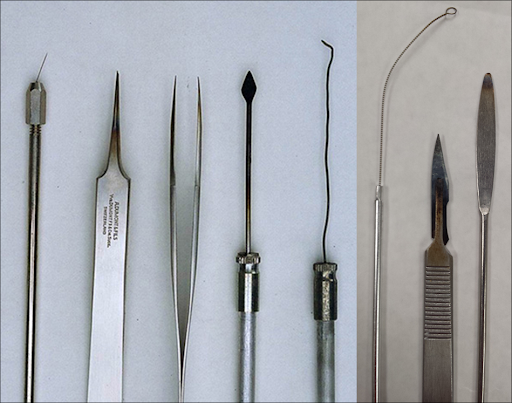
\includegraphics[width=6.83in]{img/Fig1_Ch2} 

}

\caption{ Tools used for isolating, transferring, and culturing microfungi.  From left to right: insect minuten pin with pin vice handle, two examples of fine-tipped forceps, a harpoon-like mini spatula with vice handle, nichrome wire with a vice handle, tungsten wire loop, metal-handled scalpel, and small spatula.  Fine-tipped forceps are useful for collecting segments of hyphae (e.g. for slide making or isolation in culture) whereas the insect minuten pin, nichrome wire, and loop may be used for transferring spores.  The scalpel or spatulas are needed for cutting agar plates.}\label{fig:ch2fig1}
\end{figure}

\section{Soil and Dung Collection}\label{soil-and-dung-collection}

Different taxa are commonly associated with different substrates
(e.g.~soil vs.~litter vs.~dung) so multiple substrates can be used in
order to maximize Zoopagomycotina diversity. For example,
\emph{Syncephalis} species are more common from soil samples
(\citet{Benny_2016}), whereas predaceous taxa like \emph{Zoopage}
species may be more common in decaying leaf litter
(\citet{Duddington_1955}).

\subsection{Soil Collection}\label{soil-collection}

\begin{enumerate}
\def\labelenumi{\arabic{enumi}.}
\item
  Find a location to sample. Nutrient rich and moist locations such as a
  gardens, compost heaps, beneath trees or shrubs, etc. may yield better
  results. Mesic forest habitats often yield many species of
  Zoopagomycotina.
\item
  Use a clean spoon or trowel to scoop a small amount (up to 250 mL/1
  cup) of topsoil and place in a small, clean plastic bag. If desired,
  also collect decaying leaf litter laying on the soil.
\item
  Keep soil and leaf litter refrigerated until ready to plate on media.
  (Although few studies have empirically tested the effects of
  refrigeration, anecdotal evidence suggests that fresher soil yields
  the highest diversity).
\end{enumerate}

\subsection{Dung Collection}\label{dung-collection}

Rodent and rabbit dung are rich sources of \emph{Piptocephalis} and
\emph{Syncephalis} species but isolates have also been obtained from the
dung of horses, cows, raccoons, squirrels, goats, and bats. The most
important aspect of dung collection is that it must be relatively fresh.
The dung should still have moisture and have a shiny, brown appearance.
Old dung is often drier, is white or green, and has a ``crusty''
appearance.

\begin{enumerate}
\def\labelenumi{\arabic{enumi}.}
\item
  The type of dung collected will depend on the surrounding habitat.
  Wooded areas are typically good for collecting dung from a variety of
  small mammals such as squirrel, deer, rabbit, raccoon, and mouse. Even
  arthropod dung (e.g.~cockroach or earwig) has produced some
  interesting Zoopagomycotina taxa and could be tested. Local farms with
  herbivores may be a valuable source as well. For identification of
  scats see Halfpenny (\citet{Halfpenny_2008}) or similar source.
\item
  Place the dung in an appropriate container and refrigerate until ready
  to place in a moist chamber. Firm dung (e.g.~mouse or rabbit pellets)
  should be kept in paper bags rather than in plastic bags.
\end{enumerate}

\begin{quote}
Note: Field collected dung could potentially contain nematodes or other
disease agents so it should be handled with laboratory gloves. In some
areas of the USA (e.g.~the Southwest) rodents may act vectors for Hanta
virus so it may not be appropriate to use rodent dung from all
locations.
\end{quote}

\section{Incubation of Soil and Dung}\label{incubation-of-soil-and-dung}

Two main approaches have been used to view and isolate Zoopagomycotina
species from soil and dung, incubation and plating. These approaches are
outlined briefly here.

\subsection{Soil Plating}\label{soil-plating}

\begin{enumerate}
\def\labelenumi{\arabic{enumi}.}
\tightlist
\item
  Choose a low-nutrient media plate to use for isolation. The choice of
  plate will depend on the desired fungal groups. For mycoparasitic taxa
  it is typical to use plates that include antibacterial antibiotics and
  the anti-fungal compound benomyl to reduce growth by `molds' (e.g.
  \emph{Aspergillus} and \emph{Penicillium} spp.). For predaceous fungi
  we recommend water agar plates without antibiotics or benomyl and with
  plenty of moisture. Host animals such as nematodes or amoeba are often
  more prolific if extra water is added to the plate (see Appendix below
  for agar and antibiotic recipes).
\item
  Use a spoon or small scoop to gather 1-2 grams of soil or litter and
  gently sprinkle evenly across one side of the plate (Fig.
  \ref{fig:ch2fig2}). One side of the plate is left clear of soil to
  enable easier viewing of the fungi.
\item
  Label the plate with the collection code, date, media type. Store in a
  dark cabinet or container for several days. Do {not} seal the plate
  with Parafilm.
\item
  The plates should be observed under a dissecting microscope to look
  for fungi.
\end{enumerate}

\begin{figure}

{\centering 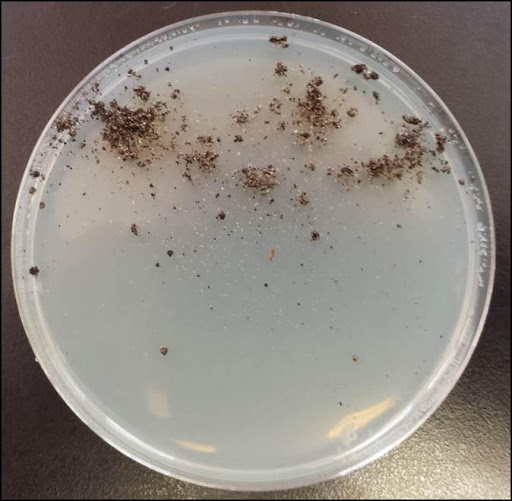
\includegraphics[width=6.83in]{img/Fig2_Ch2} 

}

\caption{ Example of a soil sample sprinkled on an agar plate.  A small amount of soil spread on half of the plate helps to minimize overgrowth of fungi as well as enable easier visualization of fungi that grow out over the agar.  This example has a minimal amount of soil, but more could be used depending on the size and consistency of the soil particles.}\label{fig:ch2fig2}
\end{figure}

\subsection{Dung Incubation in Moist
Chambers}\label{dung-incubation-in-moist-chambers}

\begin{enumerate}
\def\labelenumi{\arabic{enumi}.}
\tightlist
\item
  Plastic or glass petri dishes lined with filter paper are used for
  dung incubation. Standard size (i.e.~100 x 15 mm) petri dishes are too
  shallow for most types of dung, but may be appropriate for mouse or
  rat dung. Deeper dishes are better for allowing the growth of tall,
  aerial fungi and are best for larger dung like cow or horse (Fig.
  \ref{fig:ch2fig3}).
\item
  Divide the dung into smaller portions that will fit in the center of
  the dishes. For very small dung (e.g.~mouse), several pellets may be
  evenly spaced across the dish. The idea is to leave enough space
  around the dung for fungi of interest to grow out.
\item
  Wet the filter paper with enough distilled water to saturate the paper
  (but avoid having standing water in the bottom of the dish because
  this will promote bacterial growth). Do not parafilm the dishes.
\item
  Moist chambers can be incubated for several days before fungi appear,
  but they should be checked regularly to ensure the filter paper stays
  moist and to watch for overgrowth by other organisms (e.g.~bacteria,
  \emph{Aspergillus} and \emph{Penicillium} spp).
\end{enumerate}

\begin{figure}

{\centering 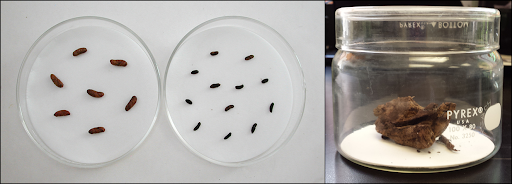
\includegraphics[width=6.83in]{img/Fig3_Ch2} 

}

\caption{Moist chamber set up for small (A) and larger (B) dung samples.  Several pellets of rat (A, left) and mouse (A, right) dung can be evenly spaced out on a standard size petri dish lined with filter paper(s).  Larger dung can be incubated in a tall glass container with a lid, also lined with filter paper(s) (B).  It is important to leave space around the dung pieces to allow room for air flow and fungal growth.  Filter papers should be wetted up to the point of saturation with distilled water and monitored to prevent dessication.  Do not Parafilm the dishes.}\label{fig:ch2fig3}
\end{figure}

\section{Viewing and Identification of Mycoparasitic
Fungi}\label{viewing-and-identification-of-mycoparasitic-fungi}

\subsection{Slide Preparation to Examine
Fungi}\label{slide-preparation-to-examine-fungi}

Slides should be made of fungi of interest for identification purposes.
Fungal hyphae can be collected with a sterilized fine instrument
(e.g.~loop) and placed in a drop of distilled water or ethanol on a
microscope slide. If using ethanol, a drop of 2\% KOH should be added to
rehydrate the hyphae. A drop of stain such as lactophenol cotton blue
may be placed next to the cover slip and allowed to diffuse across the
sample. If slides are to be kept, excess liquid should be removed from
the slide by placing a Kimwipe or paper towel beside the coverslip and
allowing it to absorb the excess. Clear fingernail polish can be applied
around the edges of the coverslip to create a seal. The area around the
coverslip should be as clean and dry as possible to ensure the polish
adheres.

\subsection{Morphological Features of Mycoparasitic
Genera}\label{morphological-features-of-mycoparasitic-genera}

\textbf{\emph{Piptocephalis}}: Common hosts: \emph{Cokeromyces,
Umbelopsis, Mucor}, and \emph{Mortierella} (Fig. \ref{fig:ch2fig4})

Morphology (Fig. \ref{fig:ch2fig5}): \textbf{\emph{Syncephalis}}: Common
hosts: \emph{Mucor, Mortierella, Zygorhynchus}, and \emph{Rhizopus}
(Fig. \ref{fig:ch2fig4})

Morphology (Fig. \ref{fig:ch2fig6}): Typically forming networks of fine,
aerial, cobweb-like hyphae; sporophores are short, unbranched, have
rhizoids at the base, and often are formed in clusters; sporophores and
hyphae are hyaline; spores are produced at the apex of the sporophores
and are usually suspended in a liquid drop at maturity; galling of host
hyphae may also be observed; zygospores have an ornamented surface and
apposed suspensors. \emph{Syncephalis} species are more common in soil
samples.

\textbf{\emph{Kuzhuaea}}: Host: \emph{Umbelopsis} (Fig.
\ref{fig:ch2fig4})

Morphology (Fig. \ref{fig:ch2fig5}): Dichotomously branched hyphae;
spores formed in zig-zag chains; zygospores ornamented with apposed
suspensors.

Molecular evidence suggests that the monotypic \emph{Kuzhuaea} is
actually a species of \emph{Piptocephalis} (\citet{White_2006}).

\begin{figure}

{\centering 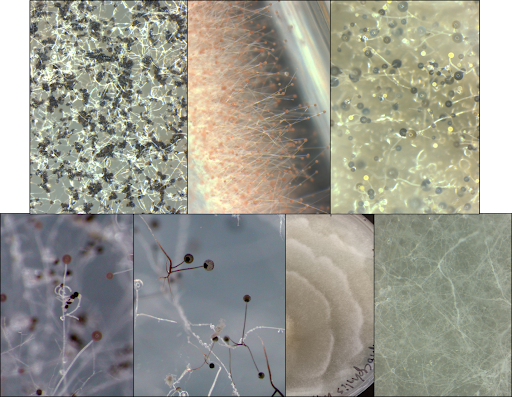
\includegraphics[width=6.83in]{img/Fig4_Ch2} 

}

\caption{Examples of common hosts for *Piptocephalis* and *Syncephalis* species.  *Cokeromyces* (A), *Umbelopsis* (B), *Mucor* (C), and *Mortierella* (F, G) are often associated with *Piptocephalis* species while *Mucor* (C), *Zygorhynchus* (D), *Rhizopus* (E), and *Mortierella* (F, G) are frequently found with *Syncephalis* species.  Species from both genera of mycoparasites are able to grow on various different Mucoromycotina hosts, and occasionally may associate with ascomycetes (i.e. *Penicillium* or *Endomyces*).  Some *Mortierella* species require special conditions in order to sporulate in culture (e.g. limited nutrients), so they may appear as masses of undifferentiated hyaline hyphae (G).  However, *Mortierella* species frequently have a characteristic zonate growth pattern on media plates (F).}\label{fig:ch2fig4}
\end{figure}

\begin{figure}

{\centering 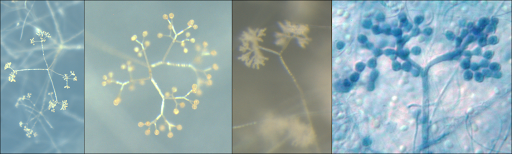
\includegraphics[width=6.83in]{img/Fig5_Ch2} 

}

\caption{*Piptocephalis* (A, B) and *Kuzhuaea* (C) under the dissecting microscope and _Kuzuhaea_ sporophores stained and viewed under the compound microscope (D).  The dichotomous branching of these species is evident.  *Piptocephalis* species typically have longer, aerial hyphae (A) that are often honey or buff colored when mature.  Some species produce spores in liquid drops when mature (B) whereas others remain dry.  _Kuzuhaea_ hyphae (C) are smaller and produce spores in chains, which can be observed under a compound microscope (D).}\label{fig:ch2fig5}
\end{figure}

\begin{figure}

{\centering 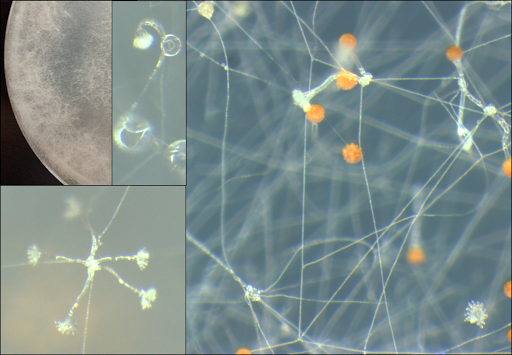
\includegraphics[width=6.83in]{img/Fig6_Ch2} 

}

\caption{*Syncephalis* species in culture.  On media plates, the presence of a *Syncephalis* species may be indicated by the tufts of fine, cobweb-like hyphae that are formed over the host (A).  Under the dissecting microscope *Syncephalis* sporophores (B, C, D) are hyaline, relatively short compared to the host (and compared to *Piptocephalis*), typically unbranched (but may be curved as in B), and sometimes are produced in clusters (C).  Red arrows indicate immature (B, C) and mature (D) sporangia.  In most species, liquid drops will form around the spores on mature sporangia.  The green arrow indicates the rhizoids that attach the sporophores to the hyphae of the host fungus.  The yellow arrow shows the fine network of thin hyphae that are produced throughout cultures of *Syncephalis* species (D).  Note: the circular objects in B are water droplets.}\label{fig:ch2fig6}
\end{figure}

\section{Isolation of Fungi from Soil and Dung
Samples}\label{isolation-of-fungi-from-soil-and-dung-samples}

If resources are available, students may try to isolate particular fungi
of interest on culture media plates. These methods are optional and
depend on the time and supplies allocated to these laboratory
activities. Isolating and culturing of fungi enable students to learn
sterile technique and further practice their microscopy skills as well
as become more familiar with microfungi morphology.

\subsection{Isolation from Soil
Plates}\label{isolation-from-soil-plates}

\begin{enumerate}
\def\labelenumi{\arabic{enumi}.}
\tightlist
\item
  For Zoopagomycotina taxa, it is necessary to include both host and
  parasite when culturing and transferring living material from one
  plate to another. Therefore, plates should be inspected under a
  dissecting microscope to locate a spot on the plate where both host
  and parasite are growing but contamination from other fungi is not
  observed. This may not always be possible, but if an appropriate site
  is found then a small section of the agar may be cut from the plate
  and placed on a new, clean plate.
\item
  Flame sterilize a small scalpel or spatula and allow to cool.\\
\item
  Carefully cut out a small square of agar where hyphae and spores of
  both the host and parasite are growing.
\item
  Using sterile technique, gently place the cut piece onto a clean media
  plate.
\item
  Try to minimize the amount of time that the lid is off the clean media
  plate in order to reduce the possibility of contamination. Remember to
  write the date and collection information on the new plate.
\item
  If there is no place on the plate where host and parasite are growing
  away from other fungi, it may be possible to isolate them using a loop
  tool or fine tipped forceps (Fig. @ref(fig:Ch2\_Fig1)).
\item
  Locate hyphae and spores of the host and parasite with the dissecting
  microscope.
\item
  Flame sterilize a tungsten wire loop or fine tipped forceps and allow
  to cool.
\item
  While looking at the fungi under the microscope, carefully touch the
  loop to the spores of the host and the parasite or grab a few
  hyphae/sporophores with the forceps.\\
\item
  Scrape the clean plate with the loop containing the spores and tissue.
  If there is difficulty in removing the tissue from the loop, it may be
  helpful to gently stab the agar with the loop. If using forceps, hold
  them vertically and stab them directly down into the agar. Try not to
  gouge or tear the agar.
\end{enumerate}

\subsection{Isolation from Incubated
Dung}\label{isolation-from-incubated-dung}

\begin{enumerate}
\def\labelenumi{\arabic{enumi}.}
\tightlist
\item
  While looking at the sample under the dissecting microscope, use a
  flame sterilized insect minuten pin, nichrome wire, or tungsten loop
  (Fig. @ref(fig:Ch2\_Fig1)) to carefully collect spores from the fungus
  of interest. If it's a mycoparasite, make sure to gather spores of
  both host and parasite. Try not to touch any other fungus with the
  tool to avoid contamination.
\item
  Stab a clean agar plate with the tool to deposit the spores. Be
  careful not to tear or gouge the agar.
\item
  Alternatively, sterilized fine tipped forceps can be used to pluck
  sporophores and place them onto a clean plate.
\end{enumerate}

These methods work well for \emph{Piptocephalis} and \emph{Syncephalis}
when they are growing on fungal hosts that grow rapidly in pure culture.
However, Zoopagomycotina (e.g.~species of \emph{Acaulopage,
Amoebophilus, Cochlonema, Endocochlus , Zoopage}) that attack small
animal hosts (i.e.~amoebae, rotifers, nematodes) will be much more
challenging to locate, identify, and maintain in dual cultures. The only
successful cultures of these fungi have been obtained when cultures of
the host nematodes or amoeba are maintained separately and inoculated
(typically with soil or leaf litter as well). For example, cultures of
the nematode \emph{Caenorhabditis elegans} may be purchased from
Carolina Biological Supply. It is also important to remember that these
fungi are often very small and may not appear on plates for weeks (or
even months), so they may not be encountered over the timeframe of a
classroom laboratory activity.

\section{Appendix 1 - Media Recipes}\label{appendix-1---media-recipes}

\subsection{Benomyl stock solution}\label{benomyl-stock-solution}

Also known as Benlate, this fungicide has low acute toxicity, but did
produce teratogenic (\citet{Cummings_1992}) and carcinogenic effects
(\citet{NRC_1987}) in rats and mice. Accordingly, personal protective
equipment including gloves and lab coat are recommended when handling
this substance. Benomyl is not soluble in water so the stock solution is
colloidal and requires shaking to resuspend the compound prior to use.

\begin{enumerate}
\def\labelenumi{\arabic{enumi}.}
\tightlist
\item
  Measure out 0.2 grams of Benomyl.
\item
  Add the Benomyl to 100 mL of sterile, distilled water. Keep the stock
  solution refrigerated. Shake or stir prior to use. (A sterile stir bar
  can be added into the bottom of the stock solution for easier and more
  even mixing of the compound).
\end{enumerate}

\subsection{Nutrient-poor media
recipes}\label{nutrient-poor-media-recipes}

Benomyl stock solution can be added at 2 mL per 1 L of media to any of
the following recipes. Benomyl is autoclavable, so it can be added
before or after sterilization. Typically, two different antibacterial
antibiotics are added after sterilization. Chloramphenicol,
streptomycin, and ampicillin are commonly used. Additional media recipes
used for different zygomycetes can be found in Benny et al.
(\citet{Benny_2016}).

{Clarified V8 juice medium} (CV8) (\citet{Benny_2016})

\begin{enumerate}
\def\labelenumi{\arabic{enumi}.}
\tightlist
\item
  Clarified V8 juice stock solution
\item
  Filter V8 juice through cheese cloth, Miracloth, or vacuum filter
  using filter paper to remove pulp.
\item
  Add powdered CaCO3 (calcium carbonate) at 3 g/L and mix.
\item
  Dilute cV8 solution with an equal volume of water.
\item
  CV8 stock solution may be aliquoted into 50 mL portions (e.g.~50 mL
  tubes) and frozen until use.
\item
  CV8 medium preparation (1 L)
\item
  Thaw one 50 mL portion of CV8 stock solution.
\item
  Measure and add 18 g agar.
\item
  Fill with 950 mL of water to reach 1 L volume.
\item
  Mix well and autoclave.
\end{enumerate}

{1/10 Wheat germ medium} (Wg10) (\citet{Benny_2016})

\begin{enumerate}
\def\labelenumi{\arabic{enumi}.}
\tightlist
\item
  Measure 3 g of wheat germ and add to 300 mL of distilled water.
\item
  Heat on hot plate or in microwave until boiling for ca. 30 seconds.
\item
  Filter solution through cheese cloth or Miracloth.
\item
  Add 0.5 g of dextrose (glucose) to the supernatant.
\item
  Add 18 g agar.
\item
  Fill to 1 L volume with distilled water, mix, and autoclave.
\end{enumerate}

{2\% Water agar medium} (WA) (\citet{Lichtwardt_1986})

\begin{enumerate}
\def\labelenumi{\arabic{enumi}.}
\tightlist
\item
  Measure 20 g agar.
\item
  Add 1 L distilled water and autoclave.
\end{enumerate}

Notes on media types and optimal usage: CV8 and Wg10 media with
antibiotics and benomyl are commonly used for soil sprinkle plates and
for isolation of fungi from mixed dung and soil cultures. These nutrient
poor media are particularly useful for obtaining cultures of
mycoparasitic Zoopagomycotina (e.g. \emph{Piptocephalis} and
\emph{Syncephalis}) because they allow for the growth of common hosts
(e.g many species of Mucoromycotina) but impair common `molds' that
belong to Ascomycota (\emph{Aspergillus} and \emph{Penicillium} spp).
However, it is important to remember that most species of
\emph{Piptocephalis} will not grow vigorously on Benomyl and the use of
Benomyl also inhibits the growth of some fungi that are known hosts
(e.g.~many \emph{Mortierella} spp.). WA is the optimum medium of choice
for predaceous Zoopagomycotina fungi and the amount of agar can be
modified as desired. The use of less agar creates a softer substrate
that amoebae can move through more easily. It is also important to be
aware of mites. Mites are common contaminates on culture plates
containing soil and leaf litter, and they can spread very rapidly from
plate to plate causing damage to the fungi you're trying to grow. To
prevent contamination of axenic or dual cultures, soil plates should be
kept in an entirely different container, cabinet, room, refrigerator,
etc. from clean plates.

\section{Appendix 2 - Preservation of Dual Host-Parasite Cultures for
Later
Use}\label{appendix-2---preservation-of-dual-host-parasite-cultures-for-later-use}

The following methods work well for medium to long-term preservation of
saprophytic zygomycete cultures in general, but specifically for
\emph{Piptocephalis} and \emph{Syncephalis} once a dual culture free
from contaminating bacteria and fungi has been obtained. Preservation
and maintenance of other Zoopagomycotina taxa that utilize small animal
hosts will require alternate methods.

\begin{enumerate}
\def\labelenumi{\arabic{enumi}.}
\item
  {Water plugs -- we recommend water plugs at room temperature for
  medium-term preservation (1-2 years maximum)}(Supp. Fig.
  \ref{fig:ch2supfig1})
\item
  Fill culture slant tubes approximately half full with distilled water
  and autoclave.
\item
  Locate areas on the plate where both host and parasite are
  sporulating.
\item
  Using a flame sterilized small circular die punch (approximately 1 cm
  in diameter) or a small spatula tool, cut the agar containing host and
  parasite into approximately 1 cm by 1cm (or 1 cm diameter) pieces.
  Very small pieces tend to revive poorly but large chunks do not fit
  well in most tubes -- be sure to adjust the size of agar blocks to the
  aperature of the tubes you are using.
\item
  Use a flame sterilized spatula or other tool to scoop the agar chunks
  up and place them into the sterilized water tube. It is best not to
  overfill the water tube, so generally around 12- 20 chunks are
  sufficient, depending on the volume of the tube.
\item
  Flame sterilize the opening of the tube when finished adding the agar
  chunks.
\item
  Replace the lid on the tube. Parafilm is recommended around the lid.
\item
  Water plugs can be stored at room temperature or in a refrigerator
  until ready to use.
\item
  When ready to revive the culture, use a sterile tool to scoop out an
  agar chunk from the tube and place on a clean agar plate.
\item
  {10\% glycerol and -80 freezer preparation -- we recommend deep
  freezing for long-term preservation (2+ years up to 10 years)}
\item
  Make and autoclave a stock solution of glycerol (10\%) and distilled
  water (90\%).
\item
  Aliquot glycerol stock solution into sterile 2 mL microcentrifuge
  tubes. Fill tubes using only 1 mL of liquid.
\item
  Locate areas on the plate where both host and parasite are
  sporulating.
\item
  Using a sterilized spatula or similar tool, gently scrape the hyphae
  of both fungi from the surface of the agar. Be careful not to puncture
  or collect any of the agar on the spatula. Collect a pea-sized amount
  of tissue, making sure to collect spores from both the host and the
  parasite.
\item
  Deposit the collected tissue into the glycerol tube and immediately
  place in a -80 freezer.
\item
  When ready to revive the culture, thaw and place the contents of the
  tube into a nutrient rich liquid medium such as MEYE (recipe below).
\item
  Once the fungi start to grow in the liquid medium, the tissue can be
  transferred to an agar plate.
\end{enumerate}

{Malt extract-yeast extract (MEYE) (nutrient rich) liquid medium}

\begin{enumerate}
\def\labelenumi{\arabic{enumi}.}
\tightlist
\item
  Measure 3 g malt extract, 3 g yeast extract, 5 g peptone, and 10 g
  dextrose.
\item
  Add 1 L distilled water and mix.
\item
  Aliquot liquid media into small slant culture tubes. Tubes need only
  be filled to approximately ½ volume.
\item
  Autoclave tubes of liquid media and store in the refrigerator until
  needed.
\end{enumerate}

\begin{figure}

{\centering 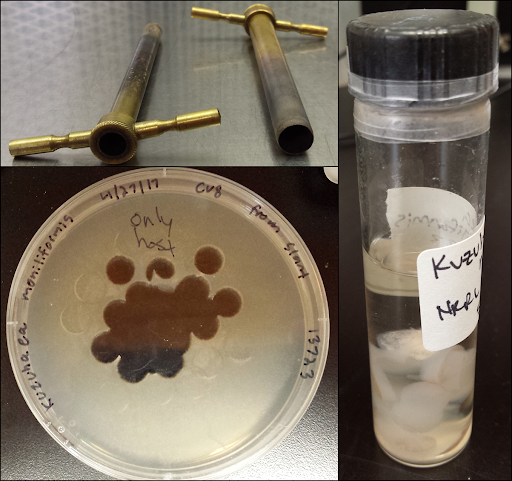
\includegraphics[width=6.83in]{img/SupFig1_Ch2} 

}

\caption{Preservation of axenic or dual cultures as water plugs.  Circular 'cork borers' (sometimes called 'die punches') (A) are helpful for cutting the agar into equally sized pieces, but a scalpel or spatula may be used instead.  Approximately 15-20 agar pieces should be cut from the culture (B) and each piece should include sporulating tissue of both host and parasite (if working with mycoparasites).  Agar chunks are placed into a labeled tube containing autoclaved distilled water and then sealed with Parafilm (C).  Water plugs may be stored at room temperature or in a refrigerator until needed. We recommend up to a maximum of two years of storage.}\label{fig:ch2supfig1}
\end{figure}

\bibliography{book.bib}


\end{document}
